\section{Aim 1. Identify allele-specific genetic interactions of the \KRAS{} alleles.}

\subsection*{Rationale}

In cancers of the colorectum, lung, pancreas, and blood plasma, \KRAS{} is almost exclusively mutated at codons 12, 13, 61, and 146, resulting in the hyperactivation of many downstream effector pathways, including, the MAPK and PI3K-Akt signaling pathways \cite{Simanshu2017}.
Many researchers believe the mutations are functionally equivalent, however biochemical, signaling, 
and clinical distinctions have been previously documented (extensively reviewed by \cite{Miller2012, Li2018}).
For example, codon 12, 13, and 61 mutations reduce the rate of intrinsic and/or GAP-mediated hydrolysis, and mutations at 13 and 61, but not 12, also enhance the rate of GDP exchange \cite{Hunter2015a, Smith2013}.
In contrast, an increased rate of GDP exchange is the only mechanism by which 146 mutations increase the concentration of GTP-bound \kras{} \cite{Feig1988RelationshipProteins., Edkins2006, Janakiraman2010, Poulin2019}.
Additional distinctions have been identified between different mutant alleles, including some between mutations at the same amino acid position \cite{Pershing2015, Hunter2015a, Poulin2019, Hobbs2019AtypicalCancer., Yuan2018, Kovalski2019, Ihle2012, Spoerner2004, Smith2014a, Pantsar2018}.
For instance, unlike the G12D/V variants, the G12R mutation does not drive macropinocytosis via a MYC-dependent mechanism in PAAD \cite{Hobbs2019AtypicalCancer.}.

Likely as a consequence of their distinct properties, associations have been uncovered between the specific \KRAS{} mutation status of a patient's cancer and its drug-response or clinical outcome \cite{Haigis2017, Li2018}.
For instance, a retrospective meta-analysis suggested that COAD tumors with a \KRAS{} G13D allele are sensitive to anti-EGFR therapies, a treatment generally discouraged for \KRAS{}-mutant tumors \cite{DeRoock2010}, likely due to allele-specific interactions with the Ras GAP NF-1 \cite{McFall2019, Rabara2019, Zafra2019}.
Another example is that the \KRAS{} G12D allele is associated with reduced overall survival in advanced PAAD when separately compared to patients with WT \KRAS{}, \KRAS{} G12R, or \KRAS{} G12V \cite{Bournet2016}.
Thus far, the hypothesis has been that the different biological properties of the mutant \KRAS{} alleles is the cause of these clinical distinctions.
However, it is also possible that allele-specific genetic interactions drive the varying clinical outcomes.

\textbf{We hypothesize that the biological distinctions between the \KRAS{} mutations result in allele-specific genetic interactions that can be used to further characterize the \KRAS{} alleles.}\footnote{The results from this analysis have been prepared for submission to \emph{Nature Genetics} as an Analysis article.}


%%%%%%%%%%%%%%%%%%%%%%%%%%%%%%%%%%%%%%%%%%%
% Aim 1.1
%%%%%%%%%%%%%%%%%%%%%%%%%%%%%%%%%%%%%%%%%%%


\subsection*{Aim 1.1. Elucidate the mutagenic origins of the \KRAS{} alleles.}


\subsubsection*{Approach}

Working with Dr. Doga Gulhan and Dr. Giorgio Melloni, mutational signatures \cite{Alexandrov2013DecipheringCancer., Alexandrov2013, Alexandrov2020TheCancer.} were used to analyze the origins of \KRAS{} mutations in previously sequenced human cancer samples from COAD, LUAD, MM, and PAAD \cite{CancerGenomeAtlasNetwork2012, CancerGenomeAtlasResearchNetwork2014, CancerGenomeAtlasResearchNetwork.Electronicaddress:andrew_aguirredfci.harvard.edu2017, Scarlett2011, Walker2019AAnalysis.}.
In brief, all single base substitution (SBS) mutations can be represented by one of the 96 possible combinations of the six pyrimidine to purine substitutions (C>T, C>A, C>G, T>A, T>C, T>G) and the flanking 3’ and 5’ bases.
Collectively, the mutations produce a 96-dimensional mutational spectrum for each tumor sample.
Signatures were discovered from these mutational spectra using non-negative matrix factorization and measured in each sample using non-negative least squares regression \cite{Alexandrov2013DecipheringCancer., Alexandrov2013}.

The association of mutational signatures with specific \KRAS{} mutations was assessed in two related ways.
First, the average levels of each mutational signature were compared when the tumor samples were grouped by cancer and \KRAS{} allele.
Second, the SBS that caused the \KRAS{} mutation and the ability of each signature to induce that mutation were used to measure the likelihood that each \KRAS{} mutation was caused by each mutagenic process.
These two methods were used to distinguish the origins of the \KRAS{} alleles.

Finally, the extent to which the active mutagenic processes in a tumor determine the distribution of \KRAS{} alleles in each cancer type was measured by calculating the predicted frequency of each allele in each tumor sample based on the frequency of mutations in the same trinucleotide context throughout the genome.


\subsubsection*{Pitfalls and alternative approaches}

One caveat to the analyses described above is that not all mutagenic forces are captured by the current array of mutational signatures.
Presently, mutational signatures are being extended to include different types of mutations beyond SBS, and we may be able to use these to enhance the above analyses.

The calculations of the likelihood that a mutational process caused a \KRAS{} allele and the estimation of the allelic distribution using the trinucleotide contexts both assume that the mutational signatures are uniformly distributed across the genome.
However, the distribution is known to be non-uniform, and instead depends on various characteristics of the DNA including the chromatin state \cite{Schuster-Bockler2012, Polak2015, Gonzalez-Perez2019} and local rate and strand-bias of transcription \cite{Tomkova2018MutationalAsymmetry}.


\subsubsection*{Preliminary data}

Using mutational signatures, we discovered that while the mutational signature burden was generally uniform across the samples of a cancer type, regardless of the \KRAS{} mutation, the likelihood of each mutational signature to have caused the acquired allele was not uniform.
For example, in COAD and PAAD, there was a higher probability of the \KRAS{} G12C mutations to have been caused by reactive oxygen species (SBS18, navy blue bars; Figure \ref{fig:mut-sig}).
Also, carcinogens in tobacco smoke were less likely to have cause the G12D allele than the G12A/C/V alleles in LUAD.

\begin{figure}[t!]
\centering
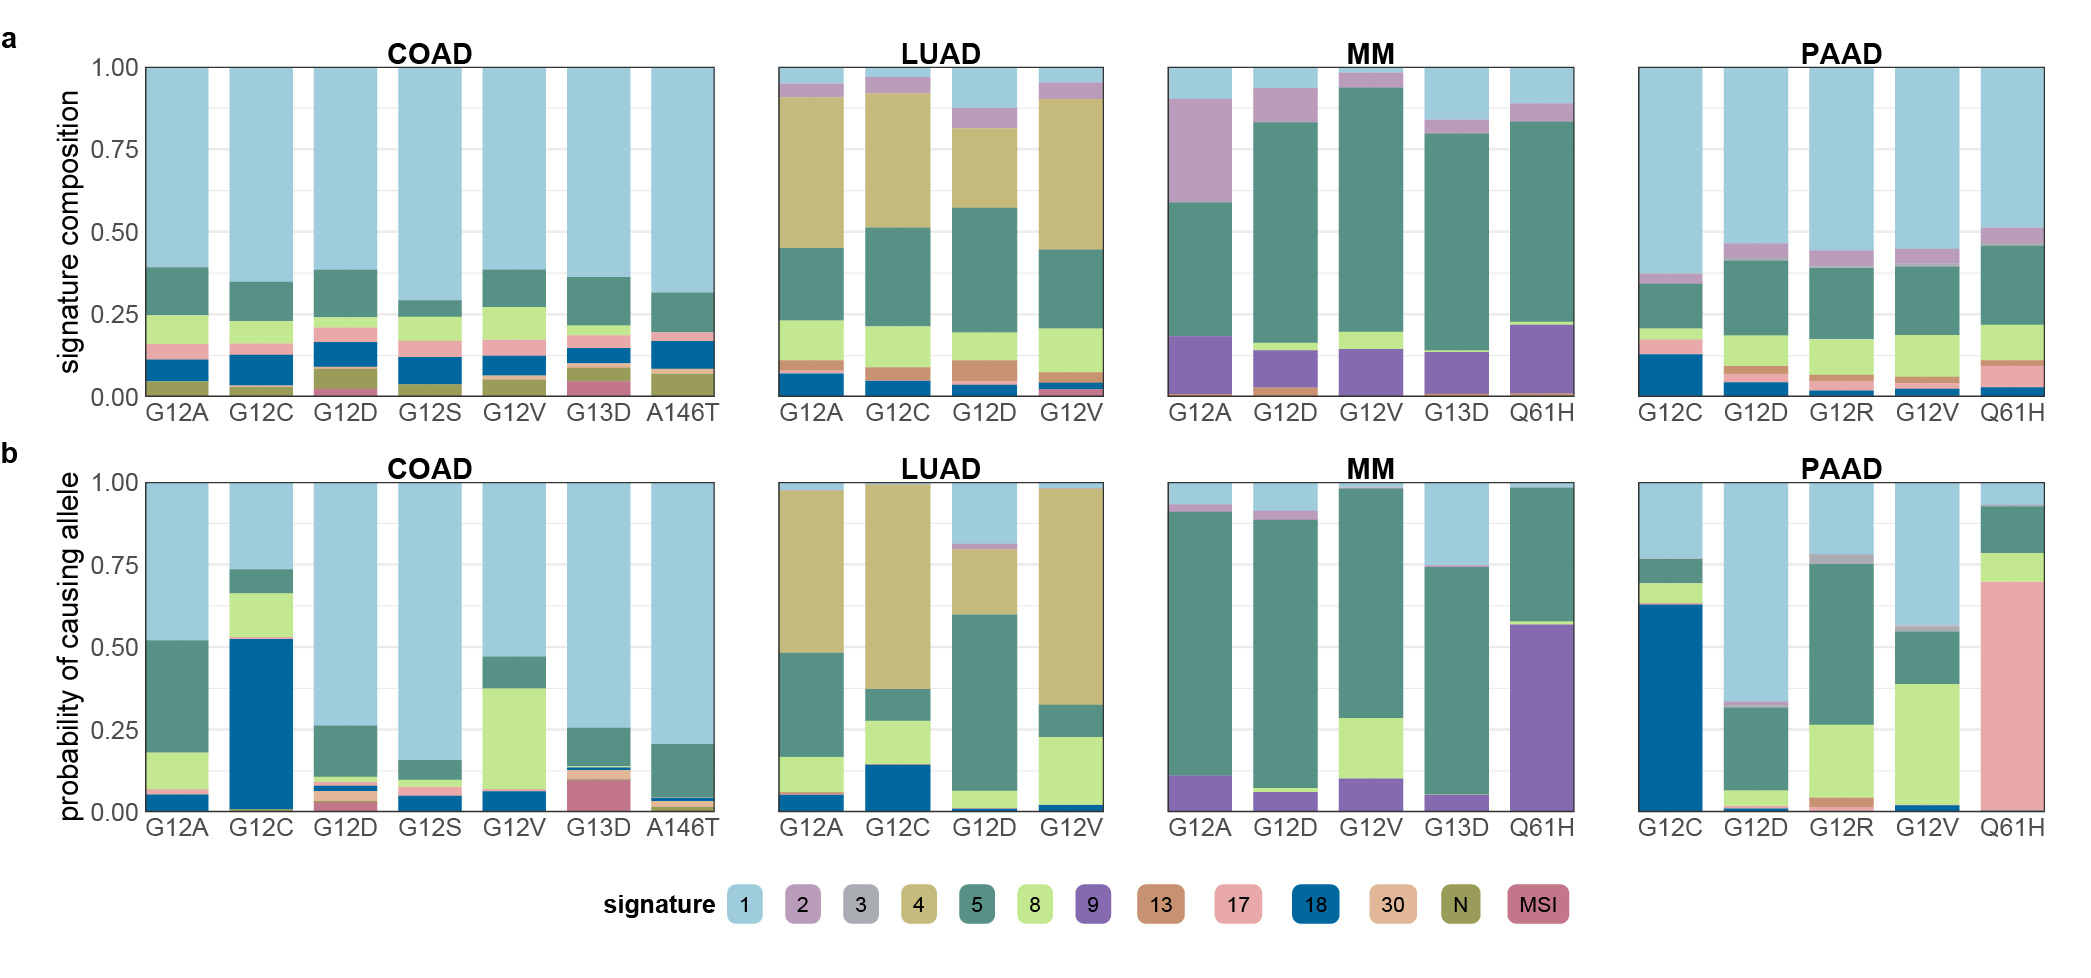
\includegraphics[width=180mm]{figures/aim1/Fig_1_mod.jpg}
\caption{
    \textbf{The contribution of mutational processes to \KRAS{} mutagenesis.}
    \textbf{a.} The average levels of mutational signatures in tumor samples separated by \KRAS{} allele. Each color represents a different mutational signature. Mutational signatures of know etiology are annotated.
    \textbf{b.} The average probability of each mutational signature to have caused the \KRAS{} mutation in a tumor sample. This value accounts for the level of each mutational signature in the tumor sample and the ability of the mutational signature to cause the indicated \KRAS{} allele.
 }
\label{fig:mut-sig}
\end{figure}

The estimates of the distribution of \KRAS{} in each cancer from the trinucleotide mutation frequencies indicated that the mutational processes in a tumor do not solely determine the \KRAS{} mutation acquired.
Figure \ref{fig:obs-vs-pred} shows the predicted frequencies against the observed frequencies of the common \KRAS{} alleles in the four cancers.
The correlation between the observed and predicted frequencies were around 0.50 for COAD, LUAD, and MM and 0.75 for PAAD.
In addition to estimating the distribution of the common \KRAS{} alleles for each cancer, a similar analysis was conducted considering all of the alleles found frequently in at least one of the cancer types (data not shown).
The alleles never or rarely found in each cancer were predicted to occur at frequencies ranging from 1.5\% (for Q61L in PAAD) to 10.5\% (for Q61K in LUAD), indicating that these alleles are not rare because their causative mutations do not occur, but instead due to weak oncogenic fitness in the tissue.
Thus, while it is likely that the active mutational processes in a tissue contributed to which \KRAS{} mutation was gained, they were not completely deterministic.
Instead, the particular biological properties of the alleles drive their selection, warranting further investigation into their genetic interactions.

\begin{figure}[ht]
\centering
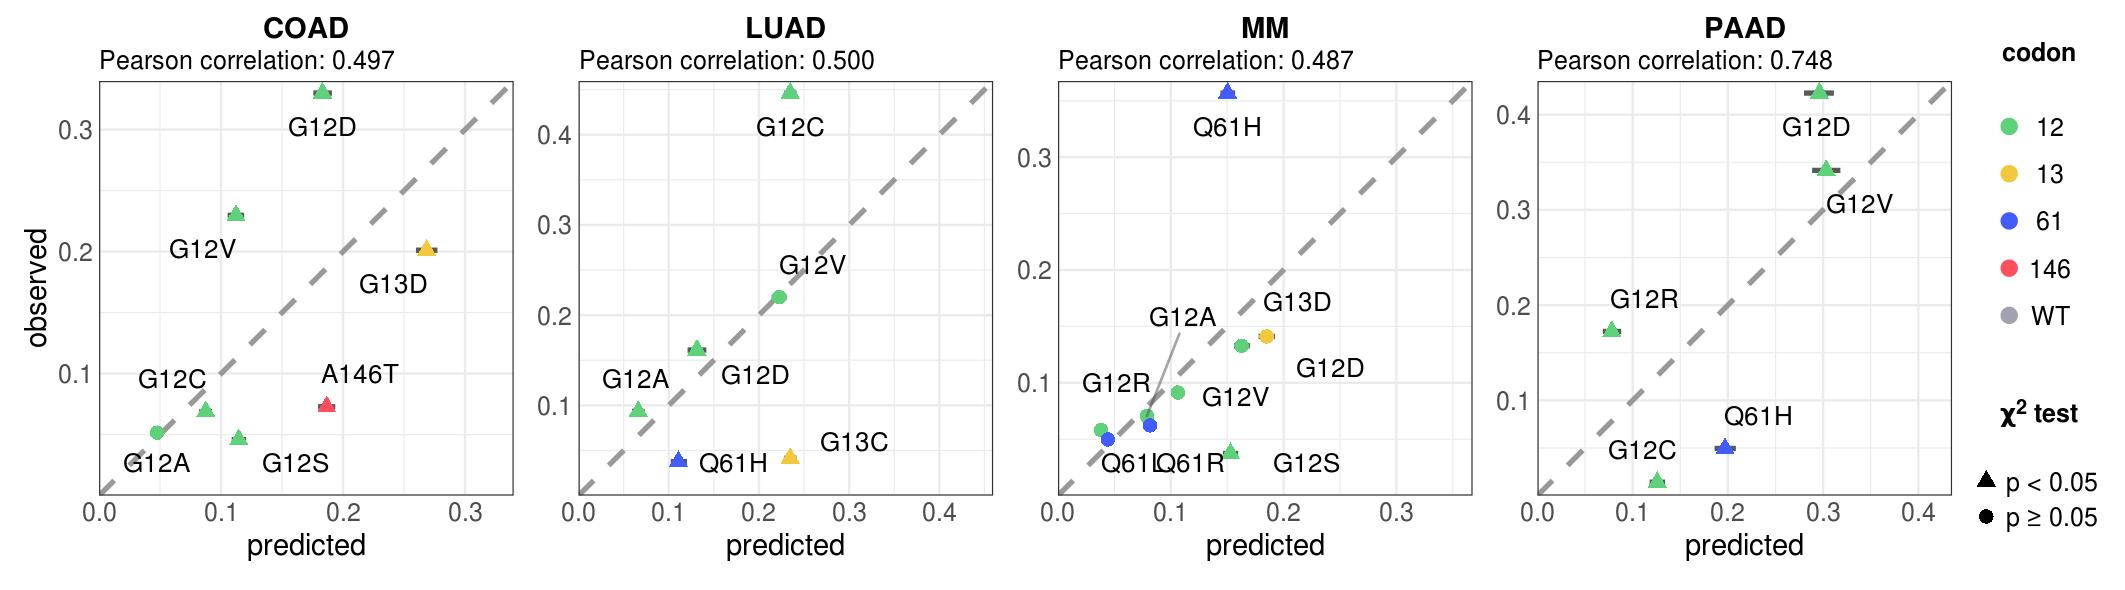
\includegraphics[width=180mm]{figures/aim1/Fig_2.jpeg}
\caption{
    \textbf{The predicted frequencies of cancer-specific \KRAS{} alleles.}
    The predicted vs. observed frequency of \KRAS{} alleles for the common alleles of each cancer. $\blacktriangle$ indicates rejection of the null hypothesis that the observed and predicted frequencies are the same (Chi-squared test, p < 0.05). $\bullet$ indicates the failure to reject the null hypothesis (Chi-squared test, p $\ge$ 0.05). Error bars indicate bootstrapped 95\% confidence intervals of the predicted values.
}
\label{fig:obs-vs-pred}
\end{figure}


%%%%%%%%%%%%%%%%%%%%%%%%%%%%%%%%%%%%%%%%%%%
% Aim 1.2
%%%%%%%%%%%%%%%%%%%%%%%%%%%%%%%%%%%%%%%%%%%

\subsection*{Aim 1.2. Discover patterns of allele-specific comutation.}


\subsubsection*{Approach}

We reasoned that if biological selection is driving \KRAS{} allele selection in cancer, then distinct functions of each mutant form of \kras{} would be reflected in cooperating genetic events. 
An increased frequency of comutation with another gene suggests a cooperative effect, whereas a reduced frequency of comutation (compared to random) suggests that the second event is functionally redundant or that it introduces an inhibitory effect\cite{Kaelin2005, Muller2015}.
The extreme of the latter effect is commonly known as "mutual exclusivity."
For instance, in COAD, \emph{APC} comutation enhances the effects of oncogenic \KRAS{}-induced hyperactivation of the Wnt signaling pathway, essential for the growth of cancer stem cells in the intestinal crypts \cite{Janssen2006, Fearon2014, Sakai2018, Jauhri2017}.
Alternatively, in LUAD, the mutational activation of \emph{EGFR} was demonstrated to be cytotoxic in the presence of a \KRAS{} mutant, and, thus, the two are rarely found in the same tumor \cite{Unni2015EvidenceAdenocarcinoma., Ambrogio2017InAdenocarcinoma.}.

To this end, the comutation interactions between each \KRAS{} allele and every other mutated gene were investigated using a one-sided Fisher's exact test of association to identify increased rates of comutation and a test for mutual exclusivity proposed by Leiserson \emph{et al.} \cite{Leiserson2016} to identify reduced rates of comutation.

To gain functional insight into the comutation networks, genes known to physically interact with \kras{} \cite{Kovalski2019}, signal up- or downstream of \kras{} \cite{Kanehisa2017, Kanehisa2016KEGGAnnotation.}, or are known oncogenes \cite{Bamford2004TheWebsite., Sondka2018} were examined further.
Also, the Enrichr tool \cite{Chen2013, Kuleshov2016Enrichr:Update.} was used to identify the enrichment of biological functions in the networks.


\subsubsection*{Pitfalls and alternative approaches}

One difficulty with the analysis was that the tumors possess passenger mutations.
To avoid these mutations resulting in false positives, only genes with an overall mutation frequency of at least 1\% in the given cancer were considered for increased comutation interactions.
In addition, only comutation partners with at least three comutation events or a comutation frequency with a \KRAS{} allele of at least 10\% (i.e. 10\% of the tumors with a \KRAS{} allele also had a mutation in the given gene) were considered.
For detecting reduced comutation interactions, only genes with a mutational frequency of at least 2\% and at least 10 mutually exclusive events (samples in which only the interacting gene was mutated or the \KRAS{} allele was present) were considered.

An additional analysis to that described could integrate the predicted effect of each mutation to the function of the gene.
There are various tools for predicting the effect of a mutation including determining patterns in the localization of the mutations to hotspots along the gene \cite{Carter2009, Dees2012, Lawrence2013, Tamborero2013, Porta-Pardo2014}, 3D-regions of the protein \cite{Reimand2013, Porta-Pardo2015, Mularoni2016, Niu2016, Tokheim2016a, Gao2017a}, and evolutionarily conserved regions \cite{Kumar2009, Adzhubei2010, Reva2011, Carter2013a, Shihab2013}.
The proposed analysis could be modified to include these scores as weights, thereby identifying comutation interactions that include mutations likely to have modified the gene's function.

Conducting this analysis in MM was hampered by the fact that this cancer is known to be frequently multi-clonal.
As such, some detectable comutation events were mutations acquired by distinct populations in a single patient, potentially obfuscating true comutation interactions.
Due to this caveat, limiting the analysis to genes known to be recurrently mutated in MM reduced the chance of highlighting a false positive \cite{Sondka2018, Lohr2014WidespreadTherapy.}.


\subsubsection*{Preliminary data}

The result of the comutation analysis on COAD, LUAD, and PAAD tumors were weakly connected networks of the \KRAS{} alleles with only a few genes linking the alleles together.
The network for COAD is presented in Figure \ref{fig:comutation-networks}a, and the subnetwork of genes known to interact or signal through \kras{} or are known oncogenes is shown in Figure \ref{fig:comutation-networks}b.
Several alleles had reduced comutation with \emph{NRAS} and \emph{BRAF} and increased comutation with \emph{APC} and \emph{PIK3CA}, interactions that have been previously documented in COAD \cite{Sensi2006MutuallyMelanoma., Jauhri2017, Seth2009ConcomitantCancer., Cisowski2016, Janssen2006, Sakai2018, Kennedy2011, Wang2013, Green2015, Yeang2008CombinatorialCancer., CancerGenomeAtlasNetwork2012}. 
Some novel interactions included increased comutation of \emph{PORCN} with \KRAS{} A146T, \emph{MTOR} with G12C, and \emph{SMAD4} with G12V.

Further, several of the alleles showed enrichment for cellular functions in their comutation networks (Figure \ref{fig:comutation-networks}c).
One of the strongest effects in COAD was an enrichment in the G12D comutation network of interactors with \emph{YWHAZ}, a 14-3-3 scaffolding protein implicated in modulating many interactions including the activity of Rho guanine nucleotide exchange factor 7 on RAC1 in phagocytosis and cell adhesion \cite{Angrand2006TransgenicSignaling.}.
Also, genes involved in the Hippo and Wnt signaling, key pathways in COAD, were enriched in the comutation networks of \KRAS{} G12V.
The comutation network of the G13D allele was enriched for genes implicated in apoptosis and senescence.

\begin{figure}[htbp]
\centering
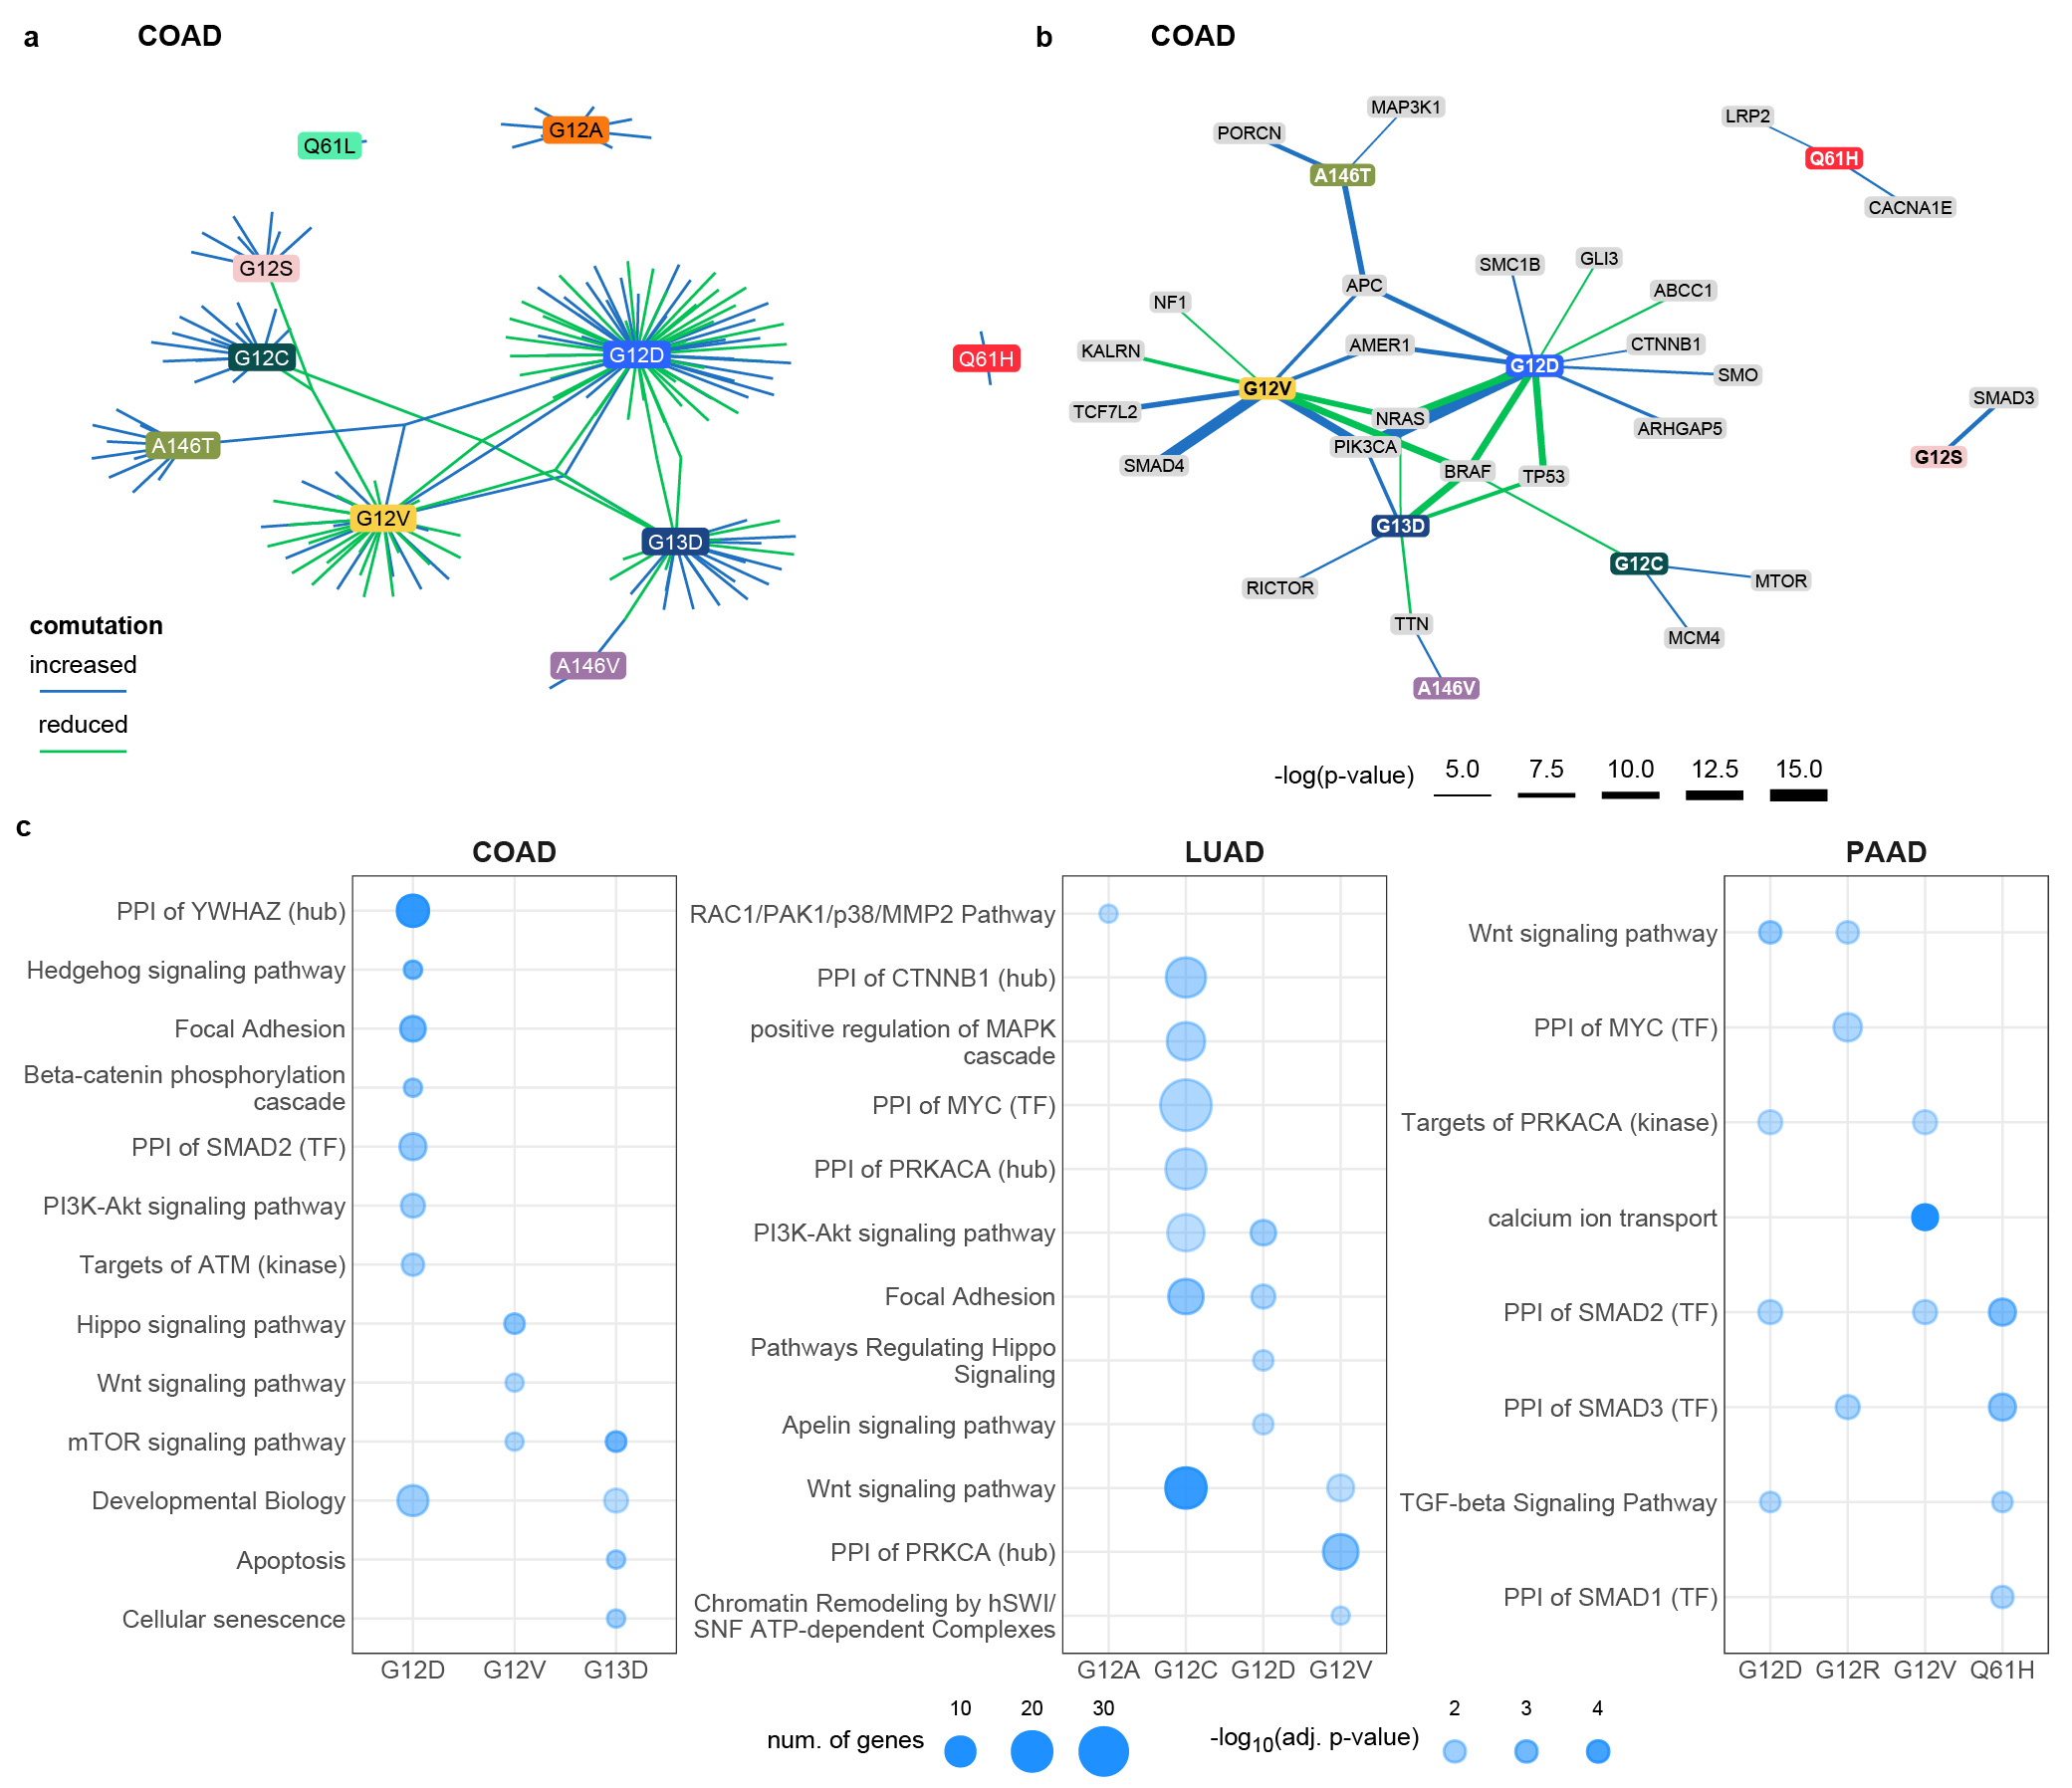
\includegraphics[width=180mm]{figures/aim1/Fig_3_mod_abc.jpg}
\caption{
    \textbf{The comutation networks of oncogenic \KRAS{} alleles.}
    \textbf{a.} The comutation network of the \KRAS{} alleles in COAD with each edge representing a comutation interaction between an allele and another gene. The color of the edge indicates whether the interaction was an increase (blue) or decrease (green) in the frequency of comutation.
    \textbf{b.} A subset of the network shown in panel a of genes that encode proteins known to physically interact with \kras{}, are in one of its canonical up- or downstream pathways, or are validated oncogenes. The width of the edge indicates the strength of the association.
    \textbf{c.} Cellular functions enriched in the comutation networks of the \KRAS{} alleles in COAD (left), LUAD (center), and PAAD (right). The size of the dot indicates the number of genes in both the function and the comutation network, and the transparency indicates the p-value of the enrichment.
}
\label{fig:comutation-networks}
\end{figure}


%%%%%%%%%%%%%%%%%%%%%%%%%%%%%%%%%%%%%%%%%%%
% Aim 1.3
%%%%%%%%%%%%%%%%%%%%%%%%%%%%%%%%%%%%%%%%%%%

\subsection*{Aim 1.3. Identify \KRAS{} allele-specific synthetic lethal interactions.}

\subsubsection*{Approach}

The perturbations necessary to drive cancer expose vulnerabilities not present in the cell-of-origin.
As the \KRAS{} alleles have measurably different signaling behaviors and genetic interactions, they likely have specific genetic vulnerabilities.
To this end, data from a genome-wide, CRISPR-Cas9 knock-out screen of cancer cell lines \cite{Tsherniak2017, Meyers2017} were used to identify genes with \KRAS{} allele-specific genetic dependencies.
The analysis was restricted to \KRAS{} alleles for which there were at least 3 different cell lines with the mutation, limiting the following investigation to only COAD and PAAD cell lines.

First, allele-specific enrichment for signaling pathways and cellular processes were identified using Gene Set Enrichment Analysis (GSEA).

Second, individual genes demonstrating differential genetic dependency by \KRAS{} allele were identified using ANOVA and one-versus-all \emph{t}-tests.
The dependency score is often linked to the expression of the gene.
Thus, when testing for allele-specific dependency of individual genes, if the RNA expression of the gene could explain the dependency score (linear model, p-value < 0.05 and $R^2$ $\ge$ 0.4), the gene was not tested for \KRAS{} allele-specific genetic dependency.
Further, genes that tended to show differential dependence on the basis of their mutation status (Wilcoxon rank sum test, p < 0.05) were not included in downstream analysis.
Of the remaining genes, an ANOVA was used to measure if the mean dependency scores for the cell lines grouped by \KRAS{} allele were different (p-value < 0.01).
For these genes, one-versus-all Student's \emph{t}-tests were used to compare the dependency scores of each group of cell lines against the others (Benjamini-Hochberg FDR adjusted p-value < 0.05).

From the results of Aim 1.2 on allele-specific comutation interactions, we posited that one or more comutating partners could be the true explanatory factors for the differential genetic dependency identified above.
This was tested by constructing linear regression models for the genetic dependency of each gene found in the above analysis with the following predictors: the RNA expression of the gene, whether the gene itself was mutated, whether the cell line had the \KRAS{} allele associated with differential genetic dependence, and one binary indicator variable for each gene that comutates (from Aim 1.2) with the associated \KRAS{} allele (Eq. \ref{eq:depmap-comut-equation}).
The model was fit with elastic net regularization \cite{Zou2005RegularizationNet}, forcing many of the coefficients to 0 to prevent overfitting.
The non-zero coefficients were individually analyzed to understand the extent to which comutation interactions may account for the measured genetic dependency.

\begin{equation}
\label{eq:depmap-comut-equation}
d_g = \alpha + \beta_{\text{RNA}}r +\beta_{\text{mutated}}m + \beta_{\text{\KRAS{} allele}}k + \beta_{\text{comutation}_1}c_1 + ... + \beta_{\text{comutation}_n}c_n
\end{equation}
\begin{equation*}
    \text{where} 
    \begin{cases}
        d_g \text{ is the dependency score from knocking-out gene $g$.} \\
        \beta_{\text{RNA}} \text{ estimates the effect of RNA expression.} \\
        \beta_{\text{mutated}} \text{ estimates the effect of a mutation to gene $g$.} \\
        \beta_{\text{\KRAS{} allele}} \text{ estimates the effect of the \KRAS{} allele.} \\
        \beta_{\text{comutation}_i} \text{ estimates the effect of a mutation to the comutation gene $i$.}
    \end{cases}
\end{equation*}

\subsubsection*{Pitfalls and alternative approaches}

One pitfall of the above analysis is that is relies on relatively few, yet diverse, cancer cell lines.
This reduces the power of the analysis to identify true allele-specific genetic dependencies.
I will work with researchers in the Haigis lab to select candidate genes for further validation in additional cell lines and other biological models such as organoids or mice.

One pitfall of the linear model proposed for modelling genetic dependency with covariates for comutation interactions is the possibility of collinearity.
This was battled via three mechanisms.
First, only comutation genes mutated in at least 3 cell lines were included as covariates.
Second, comutation genes that were perfectly correlated (i.e. they were mutated in exactly the same cell lines) were merged into a single predictor.
Third, the regularization imposed by the elastic net reduced the ability for correlated variables to inflate the variance of the coefficient estimates.


\subsubsection*{Preliminary data}

For this study, there were only a sufficient number of COAD cell lines with WT \KRAS{} and \KRAS{} G12D, G12V, and G13D, and PAAD cell lines with G12D, G12R, and G12V in PAAD.
The results for the analysis in COAD are displayed in Figure \ref{fig:genetic-dependency}.
Measuring for gene set enrichment revealed strong patterns in differential dependency of various cellular processes (Figure \ref{fig:genetic-dependency}a) including how \KRAS{} G12V cell lines demonstrated reduced dependency on genes involved in ERBB4 signaling (Figure \ref{fig:genetic-dependency}b), and the \KRAS{} G13D cell lines were less affected when genes involved in oxidative phosphorylation were targeted (Figure \ref{fig:genetic-dependency}c).

62 individual genes were found to demonstrate \KRAS{} allele-specific genetic dependency.
They were hierarchically clustered into 4 groups by their dependency scores (Figure \ref{fig:genetic-dependency}d).
Four notable genes with allele-specific associations are displayed in Figure \ref{fig:genetic-dependency}e.
First, knocking-out \emph{LIN7C}, a gene that maintains the asymmetric distribution of membrane proteins in polarized epithelial cells \cite{Monastyrskaya2013MiR-199a-5pSyndrome}, had a more severe reduction on growth in \KRAS{ } G13D cell lines compared to the others.
Also, a regulator of apoptosis previously linked to dysregulated expression in cancer, \emph{TFPT} \cite{Franchini2006ApoptosisInfluenced, Rapaport2010DeterminingCancer, Huttlin2015, Reid2019Genome-wideRisk}, demonstrated significantly greater dependency in G12D cell lines.
\emph{STARD9}, a gene encoding a kinesin required for mitotic spindle assembly \cite{Torres2011TheAssembly}, had moderate growth defects when knocked-out in all cell lines except those with a \KRAS{} G12D mutation.
Lastly, the kinetochore-associated protein (\emph{KNTC1}), a regulator of the mitotic checkpoint \cite{Chan2000HumanKinetochores., Scaerou2001TheKinetochore., Kops2005ZW10Kinetochore.}, which demonstrated moderate to strong lethal effects when knocked out in almost every cell line except for those with a \KRAS{} G12V allele.
Overall, the \KRAS{} alleles were associated with substantially different genetic dependencies on specific cellular processes, signaling pathways, and individual genes.


\begin{figure}[htbp]
\centering
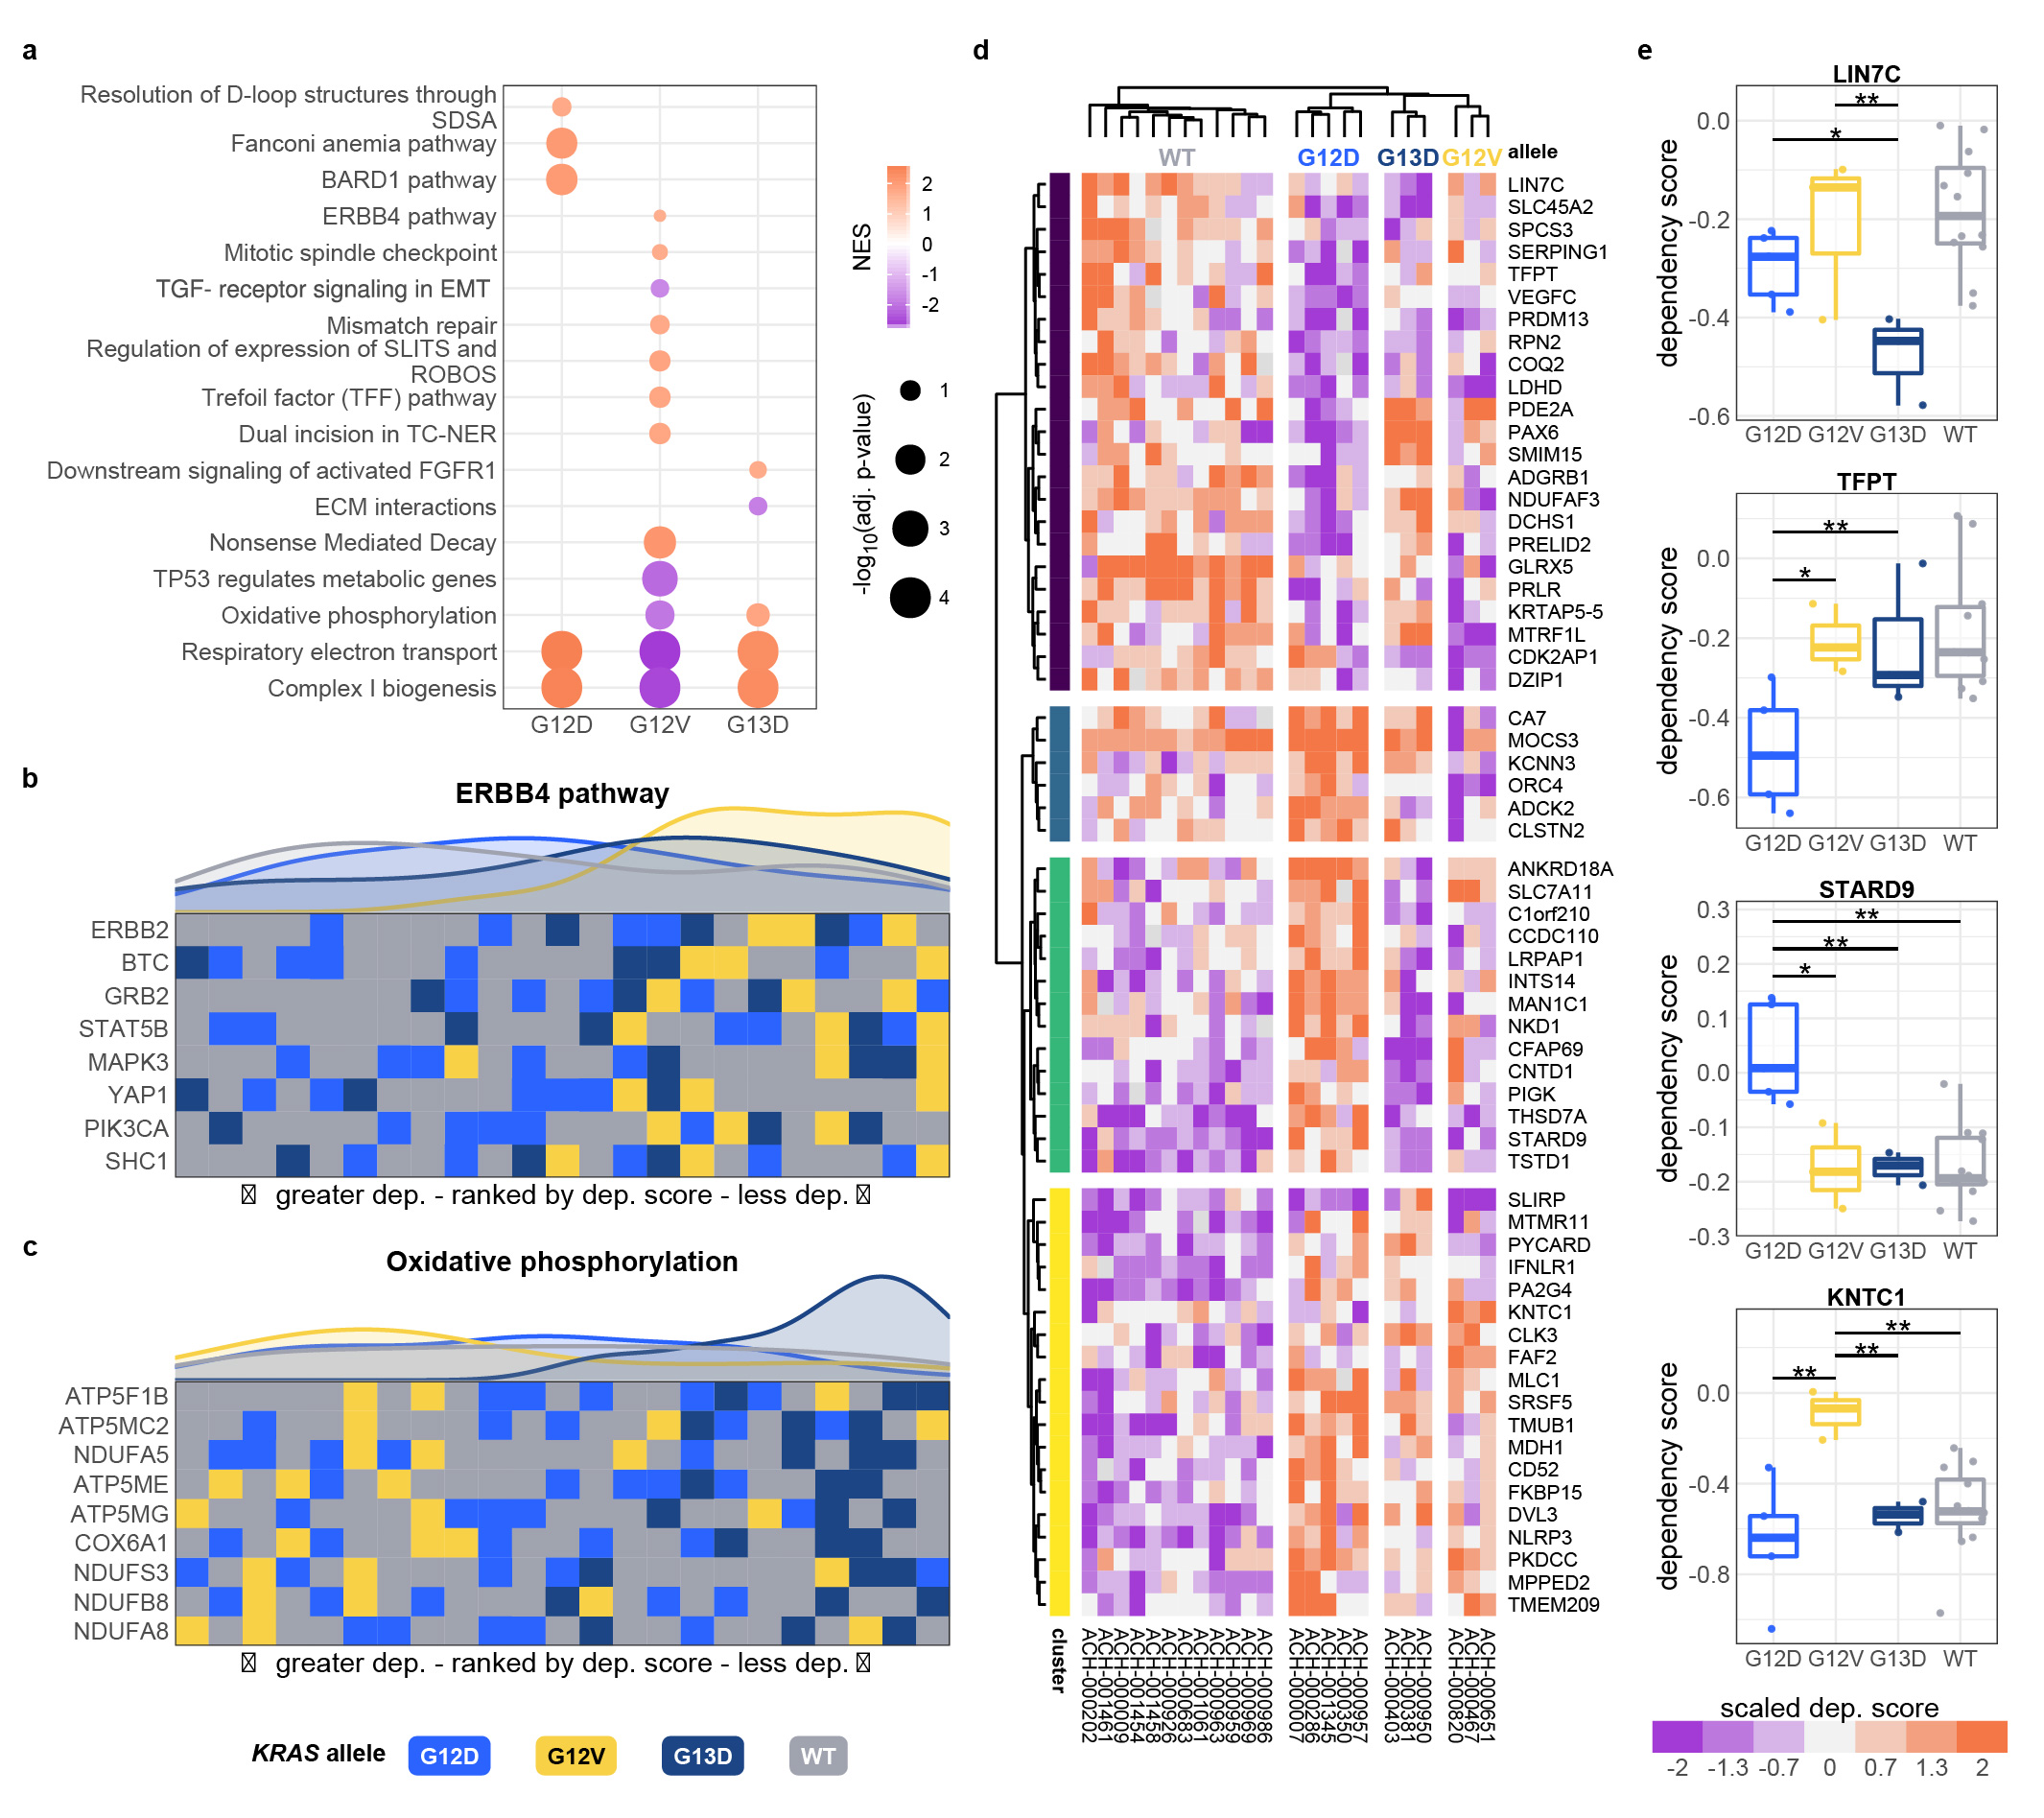
\includegraphics[width=180mm]{figures/aim1/Fig_4_mod.jpg}
\caption{
\textbf{Allele-specific genetic dependencies in COAD cell lines.}
\textbf{a.} Gene sets with significant enrichment for increased (lower dependency score; purple) or reduced (higher dependency score; orange) genetic dependency in COAD cell lines. The size of the dot relates the p-value of the association and the color indicated the strength of the enrichment ("normalized enrichment score").
\textbf{b, c.} Heatmaps ranking the cell lines by dependency score of the genes at the leading edge of enrichment for two gene sets. Each row represents a gene and each cell represents a cell line colored by its \KRAS{} allele. The cell lines are arranged in ranking order by their dependency score for the gene. Thus, each column indicates a rank. The line plots above the heatmaps indicate the representation (density) of each \KRAS{} allele at each rank across the genes.
\textbf{d.} Hierarchically clustered heatmaps of the genes that demonstrated differential genetic dependency amongst cell lines of different \KRAS{} alleles. Each column is a cell line labeled by its DepMap identifier and each row is a gene.
\textbf{e.} Examples of genes that demonstrated differential genetic dependency amongst cell lines of different \KRAS{} alleles (pairwise \emph{t}-tests; *: p<0.05, **: p<0.01, ***: p<0.001; p-values were adjusted using the Benjamini-Hochberg FDR correction method).
}
\label{fig:genetic-dependency}
\end{figure}
